\documentclass[jou,a4paper,notxfonts]{apa}
\usepackage{graphicx} 
\usepackage{palatino}
\usepackage{fancyhdr}
\usepackage{url}
\pagestyle{fancy}


% header on first page
\fancypagestyle{plain}{%
\fancyhf{} % clear all header and footer fields
\fancyhead[L]{\small
Journal of Eye Movement Research\\
1(1):1, 1-2}
\fancyfoot[C]{\thepage}
\renewcommand{\headrulewidth}{0pt}
\renewcommand{\footrulewidth}{0pt}}



\title{Distributed Eye Tracking Network for Conveying Gaze of Remote Users in a Robotic Telepresence
Scenario}
%Fill this in


%please refer to http://www.ilsp.gr/homepages/protopapas/apacls.html#titlhead for different numbers of authors and affiliations
\threeauthors{First Author}{Second Author}{Third Author}
\threeaffiliations{First affiliation}{Second Affiliation}{Third Affiliation}


\journal{}
\volume{}

\abstract{Telepresence technology permits visiting a distant geographical location using a mobile robot. A panoramic
camera on the robot can provide remote users with an immersive viewing perspective of the robot's environment.
One limitation of telepresence is that for humans around the robot or elsewhere is difficult to gather a sense of where
in the robot's environment the remote users are paying attention to. This contrasts sharply with physical presence where
body language and other subtle cues provide a hint of gaze points on space. Here, we propose the usage of a distributed
network of eye trackers to monitor the gaze behavior and field of view within the panoramic image 
of the remote subjects. The robot then superimposes the remote user's gaze behavior into a condensed 2D representation
of the panoramic image it is currently capturing. We use as an illustrative application a robot being used to visit a
museum remotely. A human museum guide directs the robot around the museum while interacting with the remote visitors.
The visualization of the remote visitors' gaze behavior provides a useful feedback signal to the museum tour guide about
the remote users areas of attention in the environment allowing online adaptations of behavior.
\linebreak \linebreak {\bf Keywords: eye tracking, gaze tracking, telepresence, eye tracking network, gaze aware
interfaces, pervasive computing, HCI, gaze responsive interfaces, human computer interaction}}

\acknowledgements{}
\shorttitle{}
\rightheader{}

% repeat the authors here (use et al if more than three authors):
\leftheader{ }

\begin{document}

\maketitle

\lhead{\small
Journal of Eye Movement Research\\
1(1):1, 1-2
}
\rhead{
Author, A., Author, B., & Author, C. (2007)\\
Short Title
}
\thispagestyle{plain}

\section{Introduction} 
Telepresence technology allows a person to feel and/or to have an effect as if they were present at a place other than
their real location. Telepresence technology requires that the remote user is provided with sensory stimuli conveying
information about the distant location in order to re-create the feeling of being in the distant location. This is
usually done via visual and audio sensors that capture and transmit the information about an environment to the remote
users. The option of interacting with the remote location through output effectors can be give to the remote users. This
can be achieved by sensing, transmitting and duplicating in the remote location the user's position, movements, actions,
or voice. Hence, in realistic telepresence sytems, information flows in both directions between the distant locations.
Telepresence systems range of possible usage scenarios have increased considerably in the last years thanks to advances
in robotics and telecommunication technologies. Among its many advantages, telepresence systems enable collaboration
independent of geographic location and provide considerable savings in terms of time, travel costs and environmental
impact for numerous usage scenarios.


A robotic telepresence system is a particular subtype of telepresence technology that allows a subject to move virtually
through a distant location by remotely controlling a wheeled robot which is usually equipped with a camera, a microphone
and a loudspeaker. A screen in the mobile robot can optionally display live video of the subject�s face allowing the
remote user to interact with subjects around the robot. 


In this work, we augment an existing telepresence system that allows remote subjects to visit a museum using a semi
autonomous mobile robot, an immersive web interface and an educator or museum tour guide near the robot which guides the
tour. The system is designed to allow remote visitors to feel as they are on an actual tour in the museum  by employing
a web browser viewer of the panoramic video streamed by the robot. The innovative part of the system is the usage of a
network of eye trackers that monitor the gaze behavior of the remote museum visitors and transmits their gaze data to
the mobile robot. The robot then displays on its on-board screen the gaze behavior of the remote users in order to
provide to the educator at the museum with a signal that conveys what is attracting the gaze (and hence the
attention) of the remote students.


The point of regard (PoR) of a computer user on the screen can be estimated using video oculography gaze tracking. The
usage of eye gaze as a pointing or control mechanism is well documented in the literature
\cite{duchowski, Rozado2012, Bonino2011, danhansenrevieweyetrackingmethods}. Gaze tracking has found a niche application
to study how computer users interact with content on a computer screen \cite{Rozado2012a, giaet, myiwann2011}. The gaze
data accumulated during a gaze tracking session can be visualized off-line as a heat map data structure. A heat map
captures the accumulated degree of attention that a given user places at different points on the screen during a gaze
tracking trial. Hence, it is well-established that the direction of gaze reflects the user's focus of attention on the
screen \cite{Zhai2003}, and hence, it provides a hint about intention. In this work, we leverage on these well known
facts about eye tracking practice and extend it to a network of eye trackers scenario used in combination to convey the
gaze behavior of several remote museum visitors in a remote telepresence systems. Since the gaze coordinates in a
remote eye tracker only reflect the PoR on a given plane, we also monitor the field of view within the panoramic video
viewer. The combination of the field of view and gaze coordinates maps to a unique point in 3D space that identifies the
position within the panoramic sphere video grabbed by the robot that is capturing the user's attention.

% Literature review
The concept of telepresence systems is not new. The work from \cite{minsky1980telepresence} coined the term
\emph{telepresence} to describe systems that would transform work, manufacturing, energy production and medicine by
allowing remote workers to carry out tasks in remote locations through the usage of robots, sensors and tecommunication
infrastructure. As a pioneer in the field, Minsky was the first to proposed the idea of being able to work in
another country or planet through remote telepresence.

One of the first and most popular applications of telepresence is videoconferencing \cite{duncanson1973video}. The
review  from \cite{Egido:1988:VCT:62266.62268} highlighted some of the limitations of the technology at the time it was
first proposed, most of which have currently already been overcome \cite{lawson2010images}.

Another branch of telepresence that has gathered a lot of attention in the research literature is telesurgery, also
known as \emph{surgery at a distance} \cite{green1995telepresence}. The technique allows surgeons to operate
robotically on a patient that is located in different geographical coordinates. Among the many benefits of
the telesurgery concept, the technology has the potential to revolutionize healthcare delivery by bringing surgical
attention to previously inaccessible settings \cite{holt2004telesurgery}.


More recently, telepresence robots that are controlled remotely and allow a human to explore remote geographical
locations have been proposed \cite{schultz1991telepresence} and have received a considerable amount of research
attention \cite{tsui2011exploring}.

An important feature of robotic telepresence systems is their ability to realistically capture their surrounding
environment in order to convey a realistic representation of their location to the remote users. Panoramic images are a
key component of many modern robotic telepresence systems. Panoramic cameras provide the functionality of capturing and
transmitting a high quality visual representation of the robot's surrounding environment. The work from
\cite{Gledhill2003435} provides a good overview of panoramic imaging technologies summarizing and comparing some of the
methods used to carry out the different steps involved in the process: capturing, image processing, image stitching, 3-D
reconstruction, rendering and visualization.


Gaze tracking has been used extensively to monitor the gaze behavior of subjects in a variety of circumstances and
environments \cite{duchowski, jacob2003eye, myiwann2011}. However, to our knowledge, there is no literature available on
the utility of using gaze tracking to transmit the gaze behavior of remote users to the robot's environment in a
telepresence system. The amount of literature on using networks of eye trackers is also very limited due to the high
cost of the devices until very recently.


In Summary, in this work, we augment a robotic telepresence system that allows live interaction between remote students
and an educator in a museum by providing the museum educator with a convinient visualization of the gaze dynamics of the
remote museum visitors. Multiple remote museum visitors connect via a single robot to the museum telepresence tour, but
each remote visitor controls their own view within the gallery. Remote students are given a tour of the museum by the
educator and can access additional digital content about objects on display through their panoramic viewers augmenting
thereby the tour experience. A network of eye tracking software in the remote students' computers monitors and transmit
their gaze behavior to the robot. This gaze behavior data is displayed in the robot screen to provide the museum
tour guide with a feedback signal about where the remote visitors are paying attention to. This information closes the
interaction loop between the educator in the museum and the remote students and offsets some of the nonverbal communication limitations of telepresence systems
by signaling to the museum tour guide where the remote museum visitors are paying attention to at any given instant in
time.


%XXXXXXXXXXXXXXXXXXXXXXXXXXXXXXXXXXXXXXXXXXXXXX
\section{Method}
The entire gaze monitoring and robotic telepresence system comprises several subparts that we described below.

\subsubsection{Eye-tracking system}
Eyes are used by humans to obtain information about the surroundings and to communicate information. When something
attracts our attention, we position our gaze on it, thus performing a \emph{fixation}. A fixation usually has a
duration of at least 150 milliseconds (ms). The fast eye movements that occur between fixations are known as
\emph{saccades}, and they are used to reposition the eye so that the object of interest is projected onto the fovea.
The direction of gaze thus reflects the focus of \emph{attention} and also provides an indirect hint for
\emph{intention}\cite{velichkovsky}.


A video-based gaze tracking system seeks to find where a person is looking, i.e. the Point of Regard (PoR), using images
obtained from the eye by one or more cameras. Most systems employ infrared illumination that is invisible to the human
eye and hence it is not distracting for the user. Infrared light improves image contrast and produces a reflection on
the cornea, known as corneal reflection or glint. Eye features such as the corneal reflections and the center of the
pupil/iris can be used to estimate the PoR. Figure \ref{screenGazeTracker} shows a screenshot of an eye being tracked by
the open-source ITU Gaze Tracker \cite{lowcostitugazetracker,Rozado2012}. In this case, the center of the pupil and two
corneal reflections are the features being tracked.


\begin{figure}[tp]
\begin{center}
 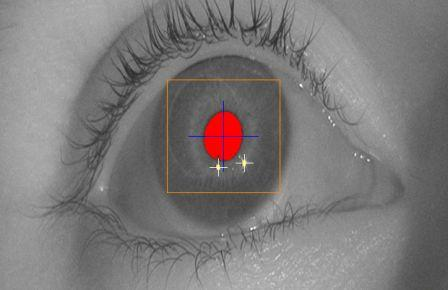
\includegraphics[width=0.45\textwidth, height=40mm]{figures/screenGazeTracker.jpg}
\end{center}
 \caption{\textbf{The Open Source ITU Gaze Tracker Tracking One Eye.} The
  features being tracked in the image are the pupil center and two corneal reflections. These features are used by the
  gaze estimation algorithms to determine the PoR of the user on the screen.}
 \label{screenGazeTracker}
\end{figure}

In most eye tracking studies, the PoR of the user is employed to generate a heat map of attention areas in the 2D scene
plane being observed or as a pointing device that substitutes the mouse in gaze interaction paradigms. For this work,
eye tracking was used behind the scenes just to capture the gaze behavior of the remote museum visitors and transmit
that data to the robot in order for it to display the aggregated gaze behavior of several users as a feedback signal to
the museum educator.

A set of 3 Tobii Rex eye trackers and 1 Tobii X1 light eye tracker are used for the experimental part. Both systems
track gaze at 30 frames per second (fps) with an average gaze estimation accuracy of 0.5 degrees at 60cm from the screen, 
\cite{TobiiTechnologyAB}. A simple exponential smoothing filter, \cite{Kumar2007}, of the raw gaze tracking data is
carried out to prevent jitter in the visualization of the remote visitor's gaze.


\subsection{Robot}
% Fred, maybe you could provide more specific and technical details about this part?
We use a commercially available Research-PatrolBot robot from Adept-MobileRobots to provide mobility and power to the system.
The robot base carries a shoulder-height Point Grey Ladybug3 panoramic camera, a touch-screen for controlling the robot and the tour, 
a web-cam for teleconferencing between the guide and remote visitors, and a computer for running the user interface and video-processing.
All data communication is over 802.11n Wi-Fi. See Figure \ref{MuseumRobot} to observe an early prototype of the system.

\begin{figure}[tp]
 \begin{center}
 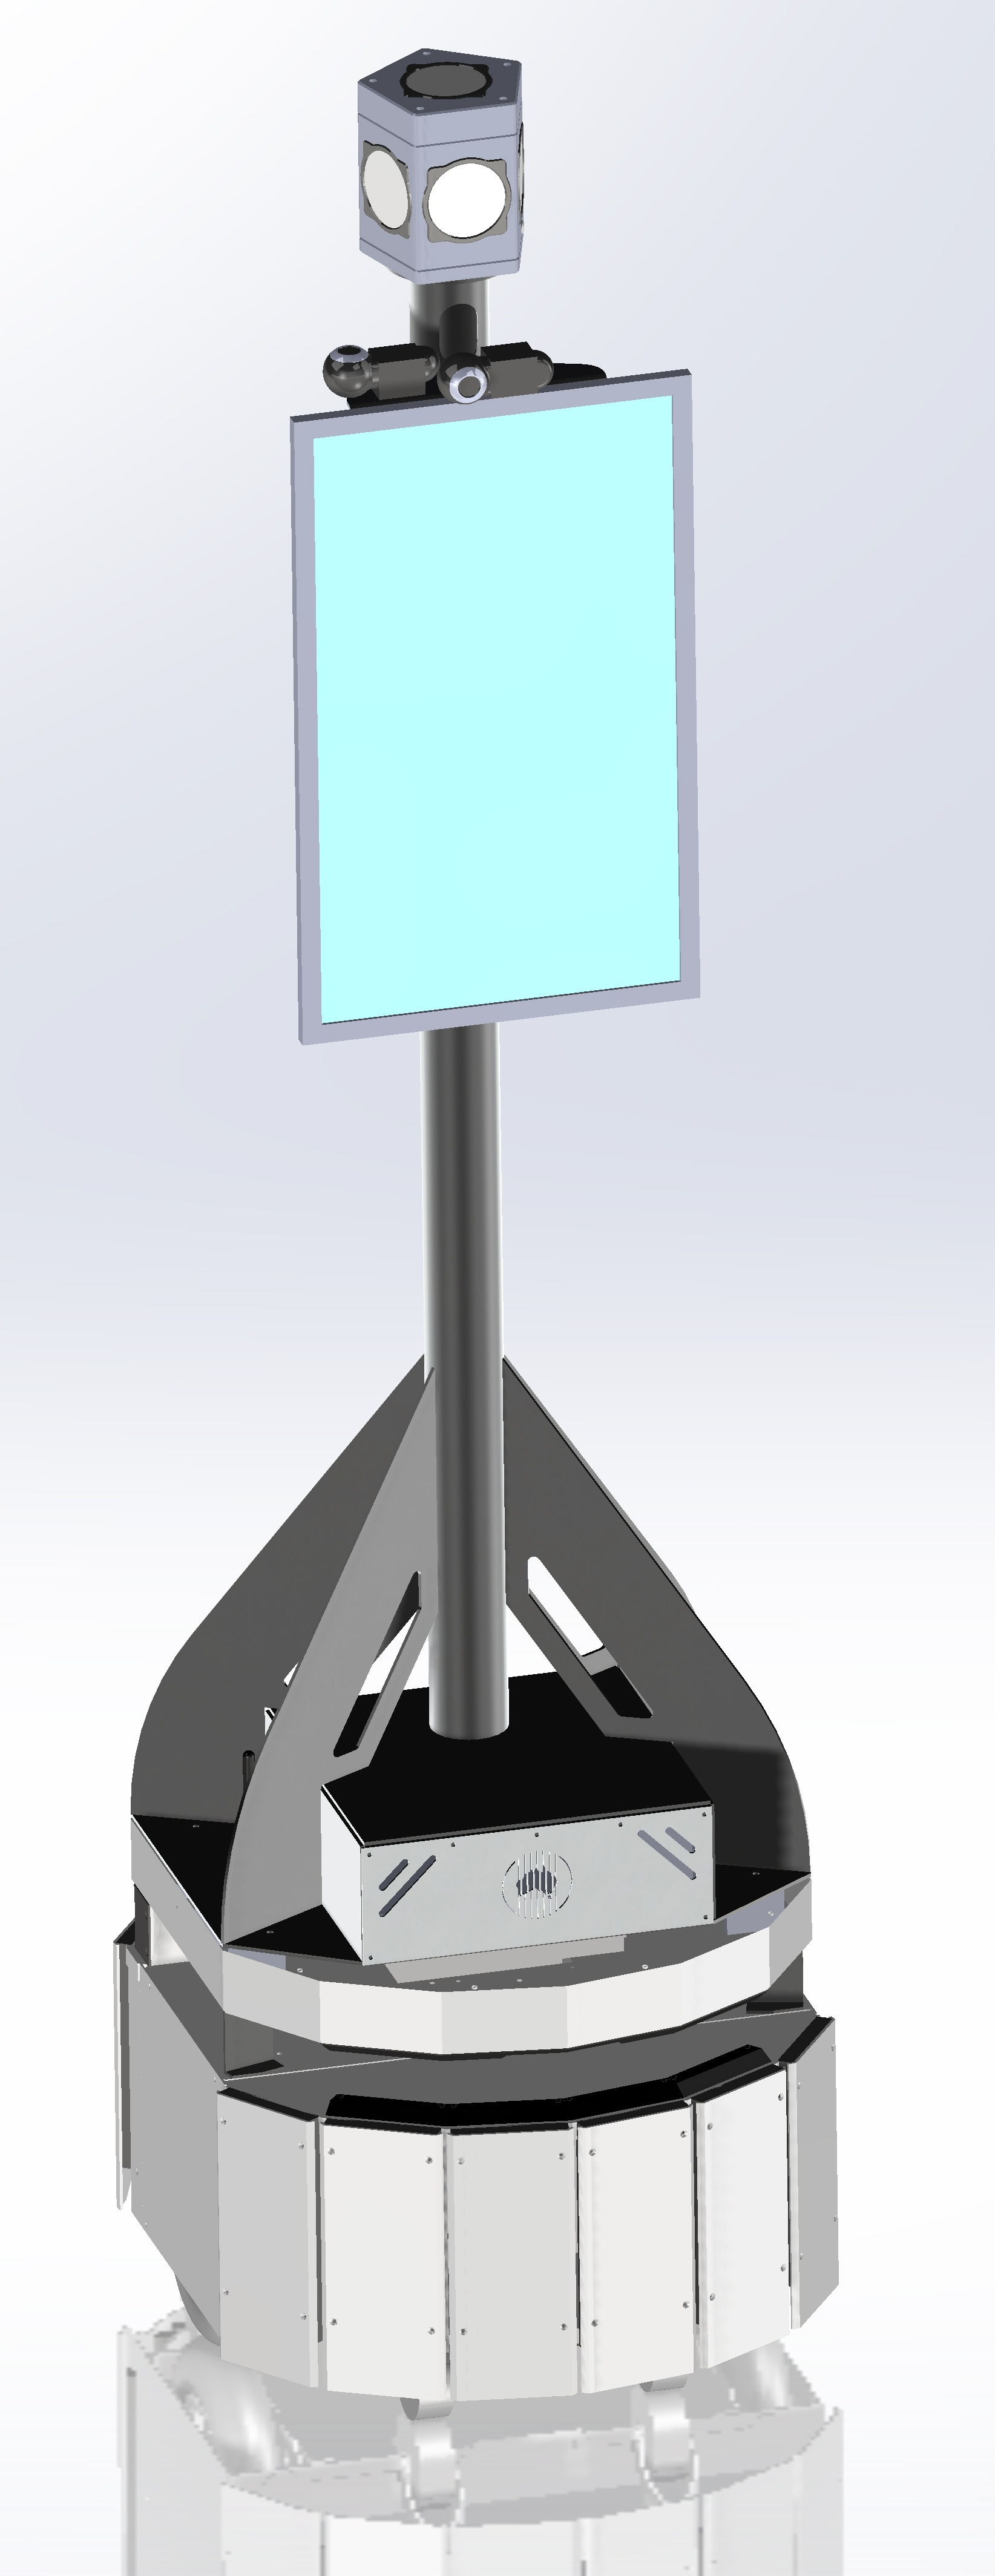
\includegraphics[width=0.25\textwidth, height=65mm]{figures/MuseumRobot.jpg}
 \end{center}
 %\fitbitmap{figures/ladybug.jpg}
 \caption{\textbf{Prototype of the Telepresence Robot.} The figure displays the main components of the robot, a
 panoramic camera on its top, a screen in the middle and a mobility unit in the bottom.}
 \label{MuseumRobot}
\end{figure}

The robot moves at walking speed within any wheelchair accessible space, and is able to navigate safely and autonomously
between pre-defined locations in the museum, as commanded by the guide. The robot navigates to a commanded destination
by first planning an efficient route within a pre-made map of the museum, and then following that route whilst reactively avoiding unmapped obstacles 
(such as people and other objects), that are detected by the on-board laser-scanner. The robot maintains an accurate estimate of its location in 
the museum by tracking its movements using wheel-odometry, and correcting for drift by matching features in the current laser scan with
features in the pre-made map.


\subsection{Museum Tour Guide}
The museum tour guide wears a wireless head-set microphone to ensure that he can be heard by the remote students while
carrying out a museum tour. The museum tour guide can see who is online and which students have questions via the
display on the front of the robot. With the proposed enhancement we are describing in this work, the museum guide is
also able to monitor the gaze of the remote visitors on the screen of the robot.


\subsection{360$^\circ$ Video and panoramic viewer}
A panorama is a single wide-angle image of the environment around the camera \cite{Gledhill2003435}. The most realistic
types surround the camera on the horizontal plane (360$^\circ$), and 180$^\circ$ in the vertical field of view. 
There are different ways to capture a panorama: single, rotated about its optical center, single omnidirectional camera
(using multiple cameras facing  in different directions) or using a stereo panoramic camera from which scene
information can be extracted.

The 360$^\circ$  panoramic camera (Figure \ref{ladybug}) used in our telepresence system was mounted on top of the robot
and captured a high-resolution omnidirectional image of the robot's environment that was further streamed to the
browser clients in the remote visitor's computers. 

\begin{figure}[tp]
\begin{center}
 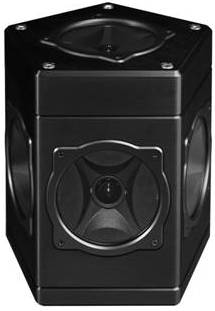
\includegraphics[width=0.25\textwidth, height=60mm]{figures/ladybug.jpg}
 \end{center}
 %\fitbitmap{figures/ladybug.jpg}
 \caption{\textbf{Panoramic Camera.} The figure displays the LadyBug3 panoramic camera on top of the robot
 that uses several cameras facing different directions to create a panoramic image of the robots surroundings.}
 \label{ladybug}
\end{figure}

The panoramic camera used in this work uses six 2.0MP cameras to capture a 360$^\circ$ by 140$^\circ$ field of view. 
The six individual images are stitched onto a fixed-radius sphere, and then mapped onto a rectangular image using a cylindrical
(Mercator) projection. A continuous sequence of these panoramic images is encoded into a high-definition video stream
and sent to each client, where it is decoded and mapped onto a spherical canvas for immersive panoramic viewing 
using a virtual camera.
(see Figures \ref{panoramicImage} and \ref{omnidirectionalimage}.

\begin{figure}[tp]
 \begin{center}
 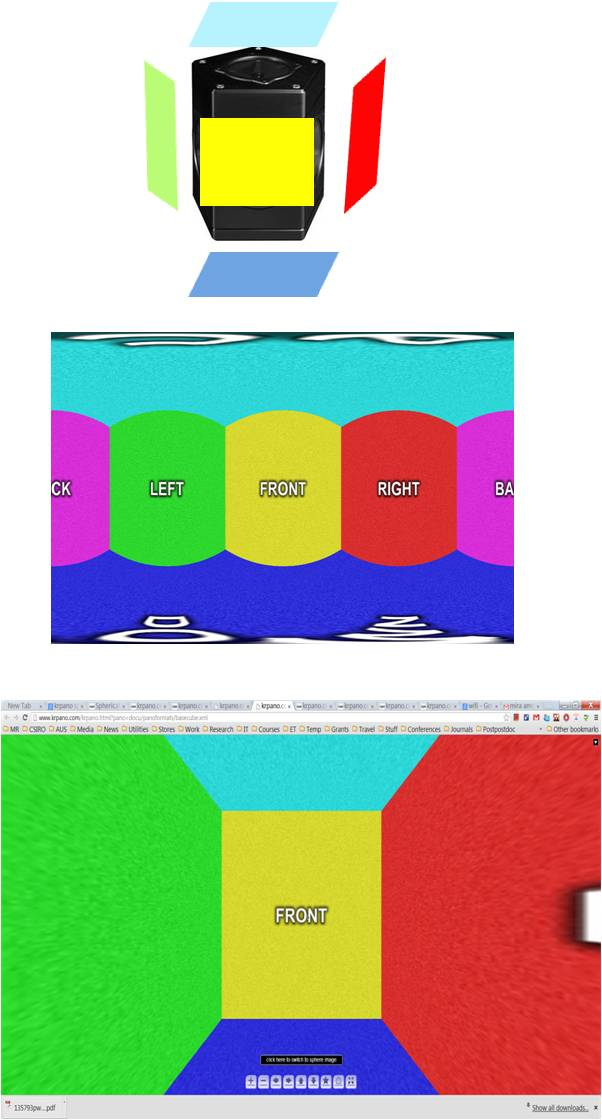
\includegraphics[width=0.48\textwidth, height=85mm]{figures/panoramicImage.jpg}
 \end{center}
 %\fitbitmap{figures/ladybug.jpg}
 \caption{\textbf{Panoramic Viewer.} The panoramic camera is used to capture different, but overlapping, views
 of the robot environment that are combined into a panoramic video stream, and sent to each client, where it is  
 wrapped onto a virtual sphere to create an immersive 3D-like experience for the remote users.} 
 \label{panoramicImage}
\end{figure}

\begin{figure}[tp]
\begin{center}
 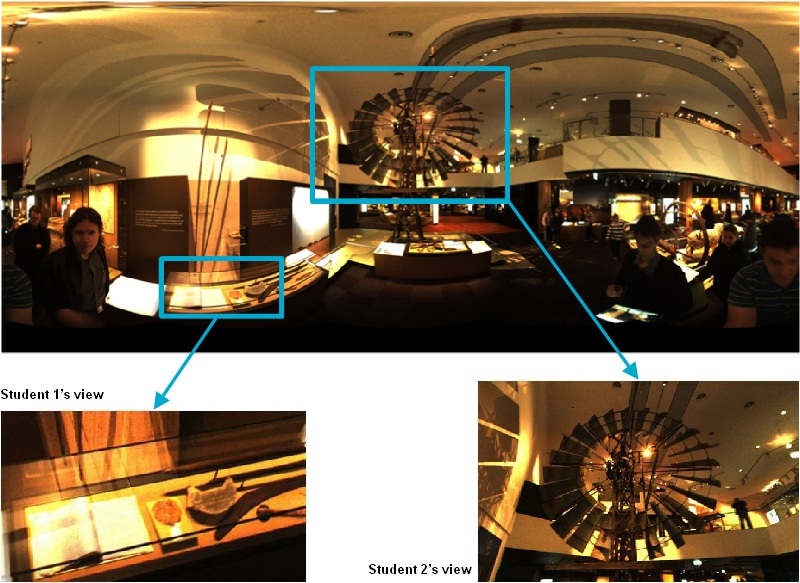
\includegraphics[width=0.48\textwidth, height=70mm]{figures/omnidirectionalimage.jpg}
 \end{center}
 %\fitbitmap{figures/ladybug.jpg}
 \caption{\textbf{Creation of an Immersive Telepresence System.} Images from the 360$^\circ$ camera on top of the robot
 are combined to form a high-resolution 2D omnidirectional image that creates a 360$^\circ$ representation of the
 environment around the robot. The image of the top of the Figure represents a condensed representation of the
 360$^\circ$ panoramic image captured by the panoramic camera. Individual users can look at different planes of the
 panoramic video stream (bottom images).}
 \label{omnidirectionalimage}
\end{figure}

We use Krpano\footnote{\url{http://Krpano.com/}} as the panoramic image viewer used in the remote computers . Krpano
is a light and very flexible high-performance viewer for all kind of panoramic images, videos and interactive virtual tours.
The viewer is available as Flash and HTML5 application and is designed for usage inside a Browser on Desktop and Mobile
computer devices. For our specific telepresence museum visit, each remote students can then independently ``look
around'' the gallery using the panoramic viewer within their browser as shown in Figure \ref{museumtourview}.

\begin{figure}[tp]
\begin{center}
 \fitbitmap{figures/museumtourview.jpg}
\end{center}
 \caption{\textbf{Panoramic Viewer in the Remote Museum Visitors' Computers.} Remote browser interface client through
 which student can look around the museum with freedom to look at different planes within the 360$^\circ$ field of view
 environment.}
 \label{museumtourview}
\end{figure}


\subsection{Remote Users' Client Computers}
Each museum visitor computer is equipped with a low cost eye tracker capturing gaze frames at 30Hz. The eye tracker
provides the X, Y coordinates of gaze on the screen plane. Since the remote museum visitor can also control their horizontal and
vertical field of view within the panoramic viewer, these parameters are also monitored by a javascript script running
behind the scenes in the browser. The horizontal and vertical view points refer to the views that determine the plane
being displayed on screen at any given time from the panoramic image. The combine parameters of horizontal and vertical
field of view and the X, Y gaze coordinates are transformed in Krpano into spherical coordinates to obtain the gaze
point of regard of the user in the spherical space. These four parameters define a unique point in the virtual 3D space
where the museum visitor is looking at and those parameters are then send back to the robot, see Figure
\ref{aggregatedGazeBehavior}.

\begin{figure}[tp]
\begin{center}
 \fitbitmap{figures/aggregatedGazeBehavior.jpg}
\end{center}
 \caption{\textbf{Eye Tracking Network.} A network of eye trackers on the remote museum visitor's computers captures the
 gaze behavior of the students. That data is combined with the specific field of view plane within the panoramic video
 stream of each student and send back to the robot. The robot then combines the gaze dynamics of each remote visitor
 with a condensed 2D representation of the omni-directional panoramic image.}
 \label{aggregatedGazeBehavior}
\end{figure}

Images from the 360 degree camera on top of the robot currently being captured are combined to form a condensed 2D
omni-directional image. The points of regard of several remote museum visitors are projected into this image to provide feedback
to the educator about where the students are paying attention to in the scene, see Figure \ref{aggregatedGazeBehavior}
and \ref{robotDisplay}.

\begin{figure}[tp]
	\begin{center}
 	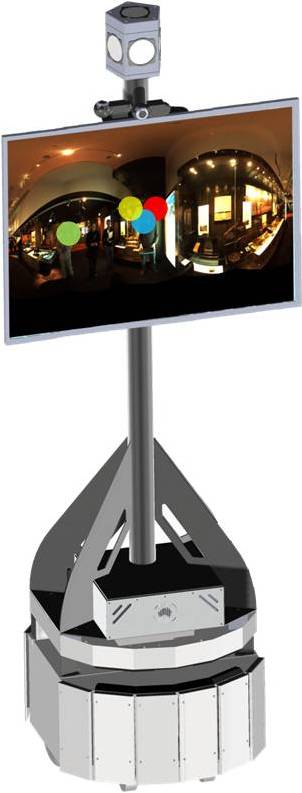
\includegraphics[width=0.3\textwidth, height=130mm]{figures/robotDisplay.jpg}
 	\end{center}
 \caption{\textbf{Visualization of Remote Museum Visitors' Gaze Dynamics on the Robot.} The aggregated gaze behavior of
 remote students superimposed into the condensed 2D omni-directional video stream is shown in the robot display so the
 tour guide can obtain feedback about what areas in the environment around the robot are attracting the visitor's
 attention.}
 \label{robotDisplay}
\end{figure}


Each remote student computer uses a server-client architecture to gather the data being monitored: gaze coordinates and
horizontal and vertical fields of view. A javascript client program embedded in the browser display monitors the
panoramic viewer field of view and stream this data through a websocket to a local server that also receives gaze
coordinates from a gaze tracker client. This server streams the horizontal and vertical field of view and the gaze
coordinates to a further server located in the robot that dispatches all the gaze data streams from different browser
clients to a handler that displays this information on top of a condensed representation 2D representation of the
omni-directional video stream currently being captured by the robot. The TCP protocol is used to issue commands to the
eye trackers such as start calibration, calculate results from calibration, start tracking, stop tracking.
Data transfers between the clients and the robot is carried out using the UDP protocol for its simplicity and due to the
fact that missing a gaze frame occasionally is not critically important for the visualization purposes. This is because
the system can afford to lose some gaze data packets since this would not impact the visualization of the gaze behavior
of remote museum visitors.

% ---------------------------------------------------------------
\section{Application}
The system described here is currently a work in progress in the prototyping stage. We are using a network of 4 eye
trackers to monitor the gaze behavior of 4 distinct users and stream that data to another computer acting as the robot
display where a condensed 2D representation of the omni-directional video stream captured by the panoramic camera is
shown. 

This work is embedded within a wider project that seeks to integrate the capabilities described here into an actual
robotic telepresence system being used by high school students (ages 10-16) to carry out remote museum visits. One of
the main features of the system is the ability of the remote students are able to customize the specific view from the
panoramic video stream that they want to take at any particular time point during the museum tour.


We have developed scripts in the browser client that stream the horizontal and vertical field of view parameters active
on each user's client computer and their gaze coordinates to a server intended to be placed in the robot. The server to
be placed in the robot receives the vector features from each connected client, parses the data and dispatches commands
to the display unit to render the gaze coordinates of each user being monitored by representing his/her gaze as a disc
over a condensed 2D representation of the panoramic image. In order to gather a sense about how the remote gaze
monitoring system in the robotic telepresence scenario works, the interested reader is encouraged to take a look at the
manuscript's associated video at \url{http://www.youtube.com/watch?v=gB89jT2_3oA}. The video provides a good visual
overview of a preliminary version of the system at work and how it can be used to monitor the gaze behavior of remote
museum visitors. The video also shows how the gaze data of the remote users is superimposed in the condensed 2D
representation of the panoramic image being captured by the robot, the key feature of the system described system. The
video shows how the museum tour guide actually moves around the museum and how she is closely follow by the
semi-autonomous robot while interacting with the students. The main contribution of the system described here to the
telepresence scenario is to provide the educator or museum tour guide with a sense of what around her catches the remote
students' attention.


An early protototype of the system described here has already been built and tested as shown in the manuscripts
accompanying video, reaching the proof of concept status. Future work will strive to carry out user studies with young
students from several national high schools in order to study their gaze dynamics during a remote museum visit by
following their gaze patterns with a larger network of low cost Tobii Rex eye trackers.


\section{Discussion and Conclusion}
Advancements in robotics and communication technologies have allowed the emergence of telepresence technology systems
that permit users to perceive and/or interact with a distant region from a remote location. The robotic telepresence
system to visit a museum described in this work is one of several examples in the growing field of robotic telepresence.
Telepresence system offer many opportunities by for instance facilitating different regions of the world to export
specialized skills anywhere at any time. The technology offers numerous additional advantages in terms of time and cost
benefits by reducing transportation costs and energy and commuting time. Last but not least, telepresence eliminates numerous chemical and physical health
hazards of physical presence in dangerous locations.


One particular are where telepresence systems can be particularly advantageous is for education scenarios such as the
system presented in this work that allows potential museum visitors such as high-school students to visit institution
with relevant education material such as museums from anywhere. National institutions such as museums have a
responsibility to reach regional and remote potential visitors who are often unable to visit them physically due to
factors such as cost and distance. A mobile telepresence system provides an opportunity for regional and remote
potential museum visitors to participate in tours on the museums and other educationally relevant institutions.


A key challenge for robotic telepresence systems for visiting distant locations through a robot will be how to leverage
the new opportunities provided by telepresence technology to engage users of the system by providing highly realistic
user experiences. In the telepresence system presented here, the panoramic viewer in the browser's client is highly
immersive and strives to make remote students feel as if they are present in the gallery through the panoramic video
stream. The systems is also highly interactive allowing remote students to select their own view within the panoramic
image and to engage in discussions with the educator and other students on the tour. The strive to make the tour a
realistic experience does not preclude augmenting the tour experience by superimposing in key objects of the museum meta
digital content layers for which a given student might wish to know more. The interactive nature of the systems
presented here in the context of a museum visit permits interactive learning rather than passive and collaborative learning by allowing
students to interact with each other and with the tour guide. This visual aspect greatly enhances communications,
allowing for perceptions of facial expressions and other body language.


However, specific telepresence application also need to overcome challenges that make the experience at its current
stage unrealistic. An important limitation of telepresence technology that we tried to bridge with our proposed system
is the lack of awareness of the humans around the robot or elsewhere about the point of regard in the environment of the
remote users. Our system bridges that gap by substituting the body language cues that actual museum visitors would provide to the
museum tour guide with a visualization of the 3D environment in 2D in the robot display where the gaze patterns of the
remote users are superimposed. The importance of high quality sensory feedback is paramount in telepresence scenarios.
The network of eye trackers system presented here provides an additional important clue to the museum tour guide about
what areas in his/her environment are attracting the student's attention.


The non-invasive nature of the eye trackers being used, by virtue of being video based and not requiring any equipment
physically attached to the museum visitors, makes them non-invasive. The gaze tracking monitoring being carried
out in the background results in a transparent user experience. Often, after the calibration the user is not necessarily
aware any more than his gaze is being monitor since the task is being carried out silently in the background.


One potential limitation of the system is the possibility of cognitively overloading the museum tour guide that while
carrying out his usual touring tasks has to pay attention to the robot's display in order to monitor where in the
environment the students are paying attention to. This potential issue can be limited by the tour guide consciously
trying to avoid continuous attention on the robot's display but rather concentrating on its traditional tasks and
looking at the display of the robot sparingly at key moments during the tour where he feels the need to obtain feedback
about the engagement levels of the tour participants.


The data gathered by the system that we proposed here is simply used to provide a feedback signal to the museum tour
guide in the current implementation, but once the capabilities to gather the data are in place, all sort of
sophisticated studies about learning during museum tour visits or other type or robotic telepresence scenarios can
be envisioned. For instance, the gaze behavior of a class of students could be monitor during the museum visit. After
the visit, the students would be required to answer a questionnaire to measure the degree of understanding and acquired
knowledge that they achieved through the visit. Using this data, looking for correlations between the gaze behavior of 
students performing poorly on the questionnaire and that of the students performing well could generate interesting
insights about the relationships between gaze dynamics and learning. This knowledge could be harnessed online to gently
push students detected to be becoming disengaged with the museum visit, in an effort to regain their attention towards
the task at hand with the end goal of maximizing the educational benefits of the museum tour. 


Any sort of large scale study looking for correlations between learning and gaze dynamics in a robotic telepresence
scenario would need a fairly large number of computers equipped with eye trackers to obtain enough statistical
significance. This could be a limiting factor in case the gaze trackers required by the proposed method would be
expensive. However, we reckon that low end eye trackers providing 30 frames per second tracking performance and the
standard reported average accuracy of 0.5 degrees at 60 cm from the screen should suffice for numerous analysis and
experimental scenarios. The current trend towards lower cost eye trackers from major manufacturers suggests that eye
trackers hardware costs will not be a limiting factor for this sort of research.

 
In summary, the system presented here is first of its kind in capturing the gaze data of several remote museum visitors
in a robotic telepresence scenario in order display their gaze activity to a museum tour guide. This important feedback
signal helps to bridge the communication gap between the museum tour educator and the distant museum visitors. Further
studies should build over the here proposed system and use the gaze data generated by the system to find
out those students that are not benefiting from the museum tour and provide them with online signals to recapture their
attention dynamically in order to improve their educational value of the museum visit experience.


\bibliography{library}
\end{document}

